\documentclass{article}
\usepackage{../../Self_Style}

\title{Phys 20AL Week 8: Path of Light}
\author{Zih-Yu Hsieh}
\date{\today}

\begin{document}
\maketitle

\section{Aim for the Experiment}
The aim for the experiment is to study the path that light travels: First it'll be focused on using Snell's Law to calculate a half-cylinder's index of refraction (that's independent of the frequency of the light). Later on it'll be focused on using the prism to get a frequency-dependent index of refraction for a prism instead.

\section{Experimental Setup}
The equipments include: A light source (with both white light, and RGB lights), a protractor, and transparent half-cylinder and triangular prism.

The equipment setup is also simple: setup the light so the path of the light passes through where the half-cylinder and the triangular prism are going to be at, and put a protractor below.
\begin{figure}[h!]
    \centering
    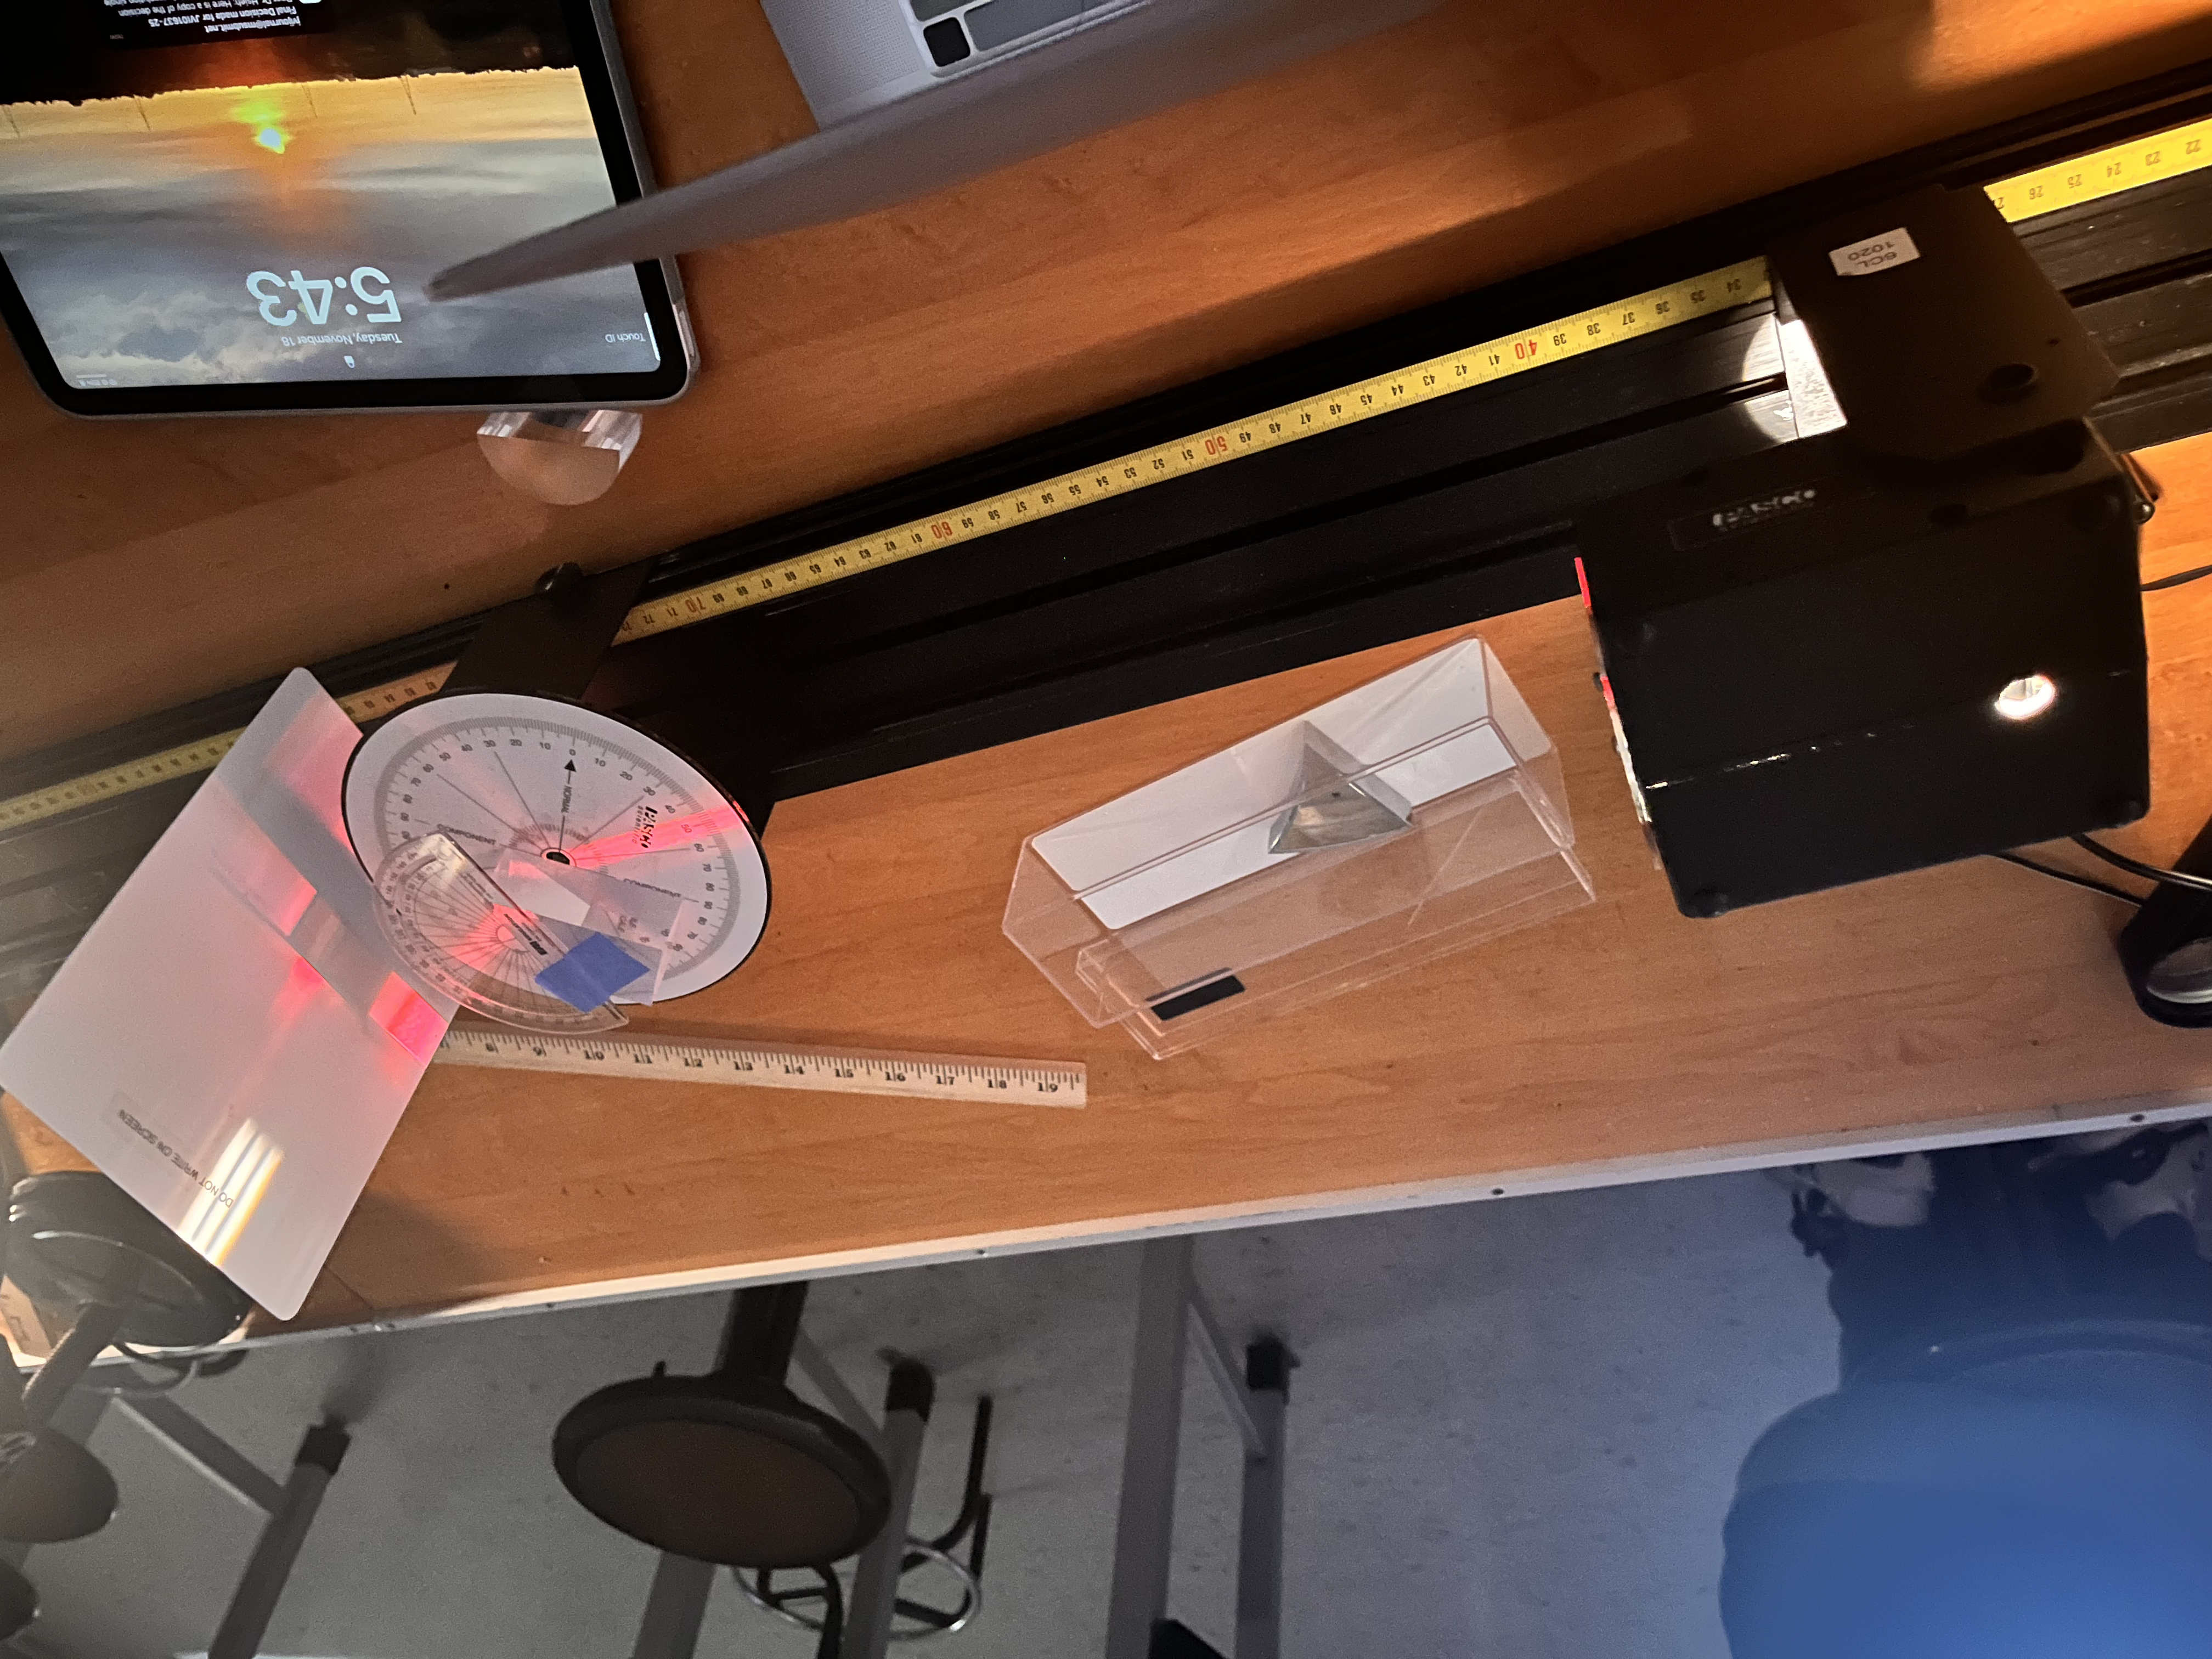
\includegraphics[width=100mm]{lat_setup8.png}
    \caption{The actual lab setup picture}
\end{figure}

\section{Quantity to Measure \& Method of Measure}
For measuring the index of refraction through Snell's Law, the incident angle of the light away from the normal line of the surface well be measured (for both the input and output light), and it'll be measured through the protractor.

For both experiments (using the white light and the RGB light), there are total of $5$ incident angles: $10,20,30,40,50^\circ$ that are used as manipulated variable. For the second experiment specifically (the RGB light one), the color (or frequency) of the light is also a manipulated variable.

For each pair of manipulated variables, total of 3 trials fo measurement will be performed.

\hfil

\section{Experimental Procedure}
\subsection{Frequency Independent Experiment}
It'll follow the procedure below:
\begin{enumerate}
    \item Turn on the white light, and put the half-cylinder on the path of the light, with the flat side facing toward the light.
    \item Tweak the cylinder, so the light is passing directly through the center of the half-cylinder (or, the center point of the semicircle).
    \item Adjust the angle of the cylinder, so the light has incident angle as one of the angles to be measured. Then, measure the incident angle of the output light.
    \item Repeat Step 3 for all the other angles await to be measured.
    \item Repeat Step 3-4 for a total of 3 trials to get all the desired measurements.
\end{enumerate}
Afterward, using the gathered data to calculate the index of refraction of the half-cylinder, use it to predict the critical angle, and test how well the prediction is experimentally.

\subsection{Frequency Dependent Experiment}
In this case, the experimental procedure is quite similar to the previous one, except now there are 3 different light sources - red, green, and blue. So, the experiment described above needs to be repeated for all types of light source, to get the index of refraction with respect to each frequency of light.

\section{Experimental Data}
The experimental data for each is as follow:
\subsection{Frequency Independent Experiment}
\begin{figure}[h!]
    \centering
    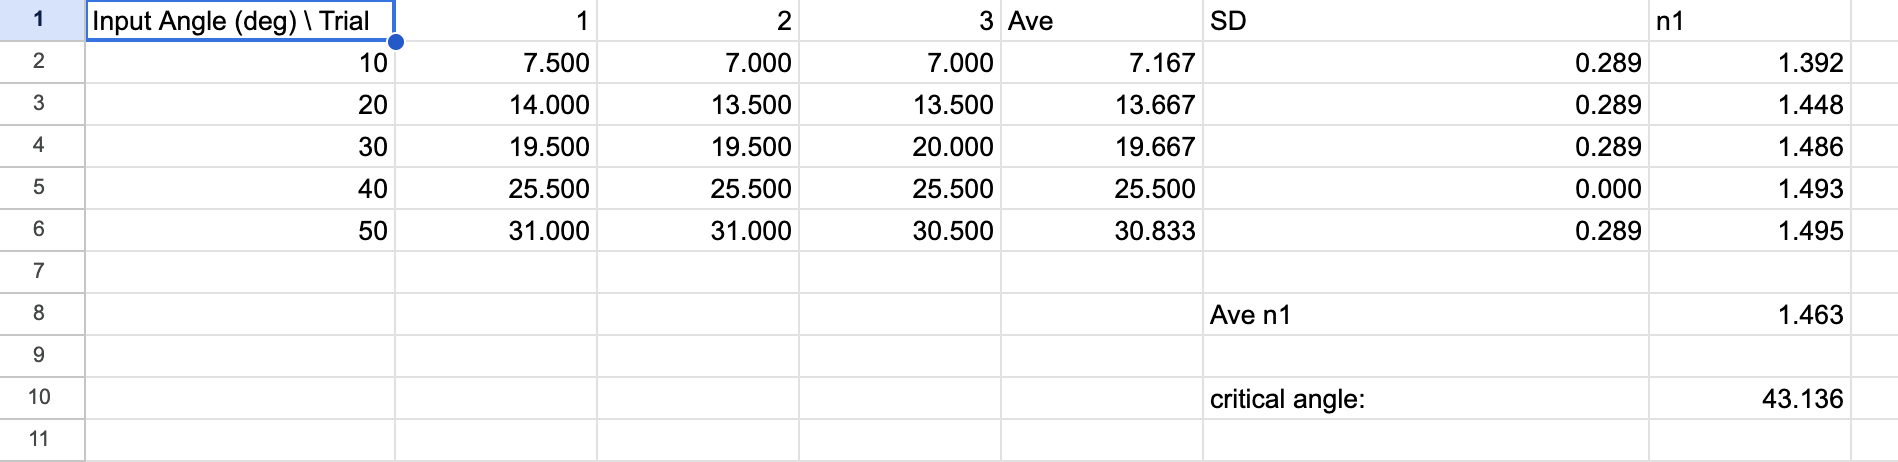
\includegraphics[width=150mm]{indep_data.png}
\end{figure}
\begin{figure}[h!]
    \centering
    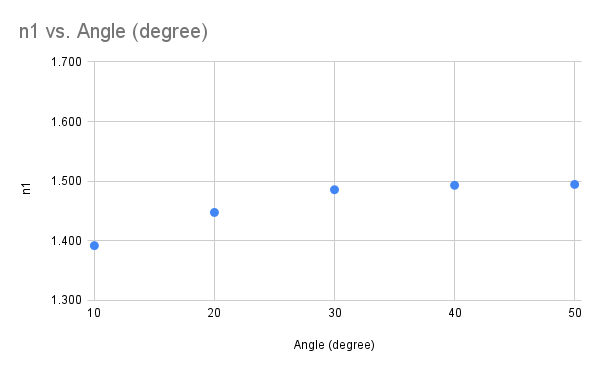
\includegraphics[width=100mm]{n1 vs. Angle (degree).png}
\end{figure}

\newpage

\subsection{Frequency Dependent Experiment}
\begin{figure}[h!]
    \centering
    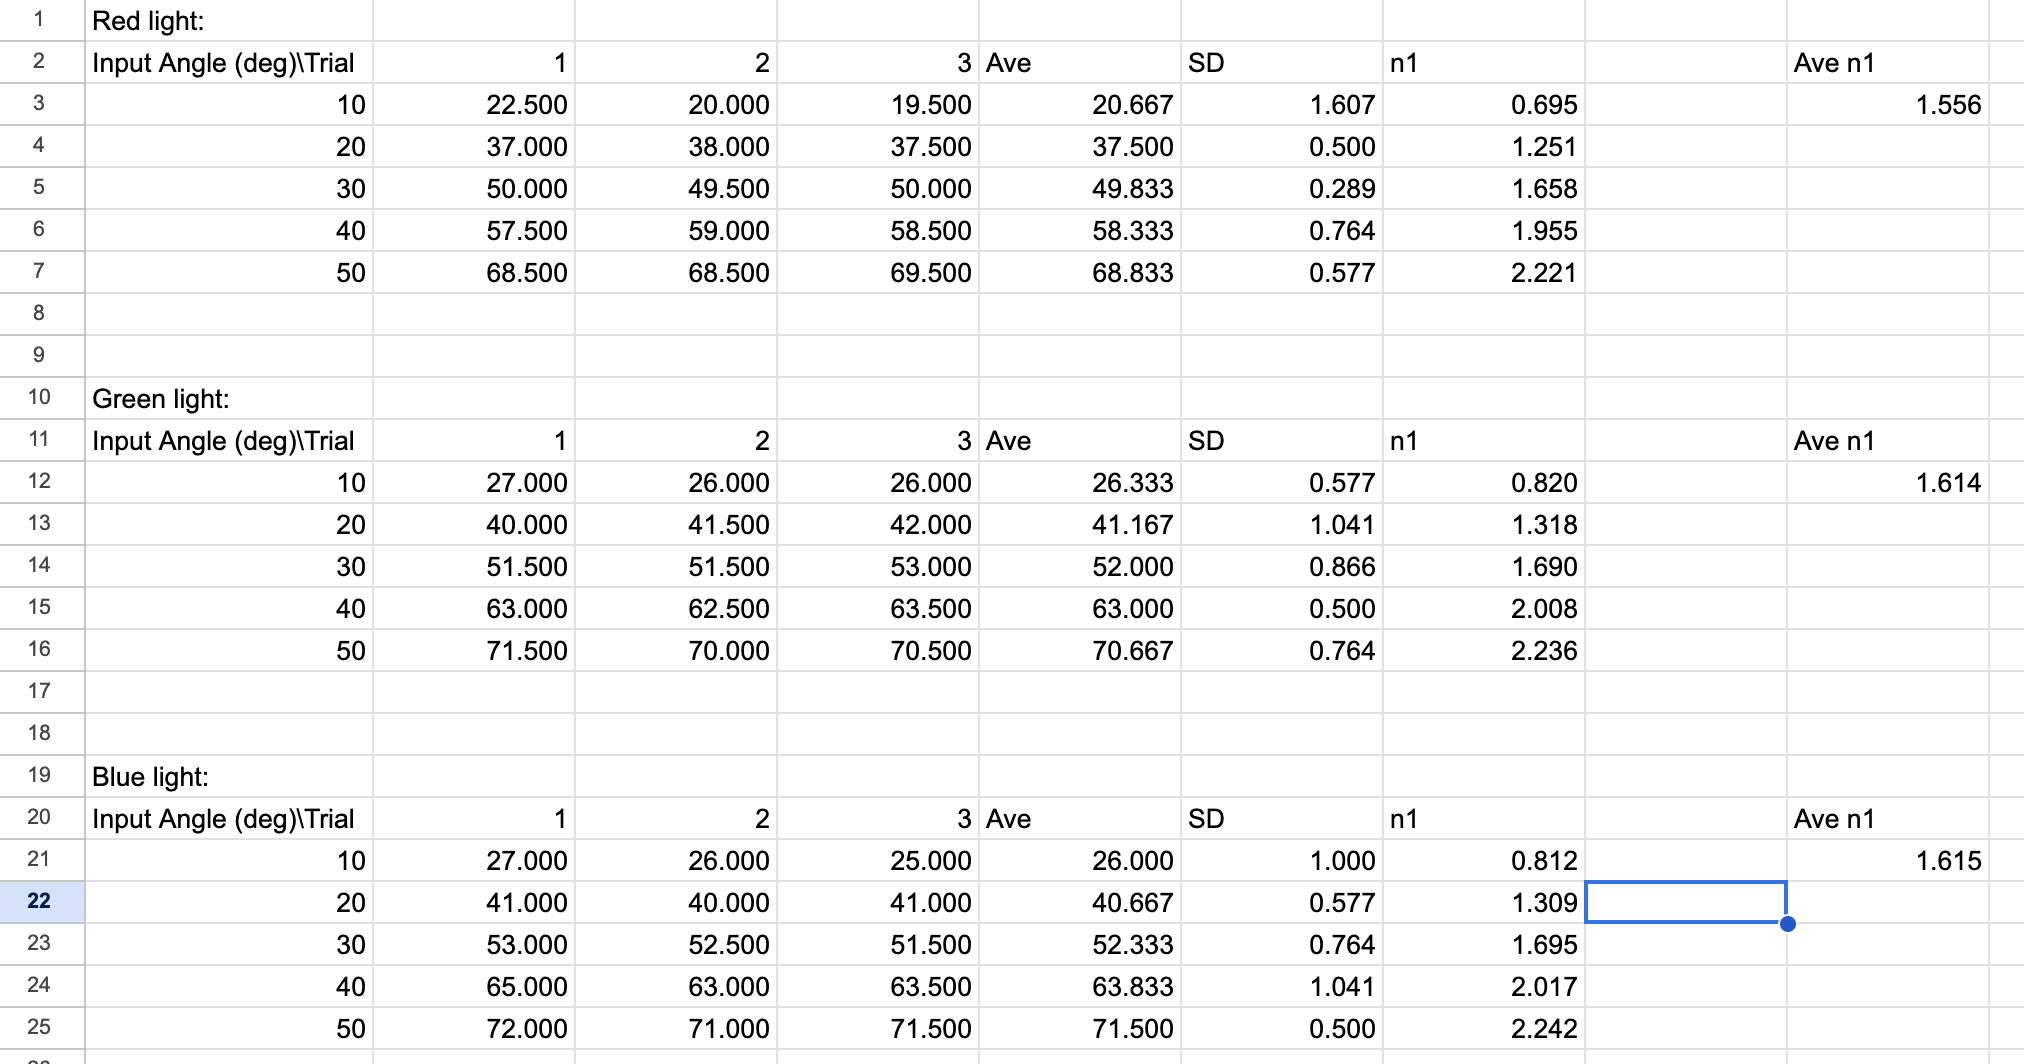
\includegraphics[width=150mm]{dep_data.png}
\end{figure}
\begin{figure}[h!]
    \centering
    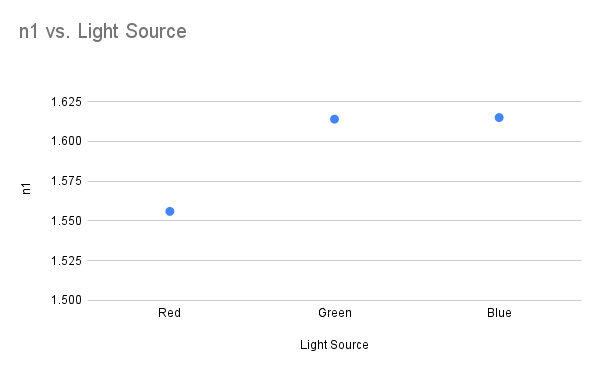
\includegraphics[width=100mm]{n1 vs. Light Source.png}
\end{figure}

\end{document}